% GNUPLOT: LaTeX picture with Postscript
\begingroup
  \makeatletter
  \providecommand\color[2][]{%
    \GenericError{(gnuplot) \space\space\space\@spaces}{%
      Package color not loaded in conjunction with
      terminal option `colourtext'%
    }{See the gnuplot documentation for explanation.%
    }{Either use 'blacktext' in gnuplot or load the package
      color.sty in LaTeX.}%
    \renewcommand\color[2][]{}%
  }%
  \providecommand\includegraphics[2][]{%
    \GenericError{(gnuplot) \space\space\space\@spaces}{%
      Package graphicx or graphics not loaded%
    }{See the gnuplot documentation for explanation.%
    }{The gnuplot epslatex terminal needs graphicx.sty or graphics.sty.}%
    \renewcommand\includegraphics[2][]{}%
  }%
  \providecommand\rotatebox[2]{#2}%
  \@ifundefined{ifGPcolor}{%
    \newif\ifGPcolor
    \GPcolorfalse
  }{}%
  \@ifundefined{ifGPblacktext}{%
    \newif\ifGPblacktext
    \GPblacktexttrue
  }{}%
  % define a \g@addto@macro without @ in the name:
  \let\gplgaddtomacro\g@addto@macro
  % define empty templates for all commands taking text:
  \gdef\gplbacktext{}%
  \gdef\gplfronttext{}%
  \makeatother
  \ifGPblacktext
    % no textcolor at all
    \def\colorrgb#1{}%
    \def\colorgray#1{}%
  \else
    % gray or color?
    \ifGPcolor
      \def\colorrgb#1{\color[rgb]{#1}}%
      \def\colorgray#1{\color[gray]{#1}}%
      \expandafter\def\csname LTw\endcsname{\color{white}}%
      \expandafter\def\csname LTb\endcsname{\color{black}}%
      \expandafter\def\csname LTa\endcsname{\color{black}}%
      \expandafter\def\csname LT0\endcsname{\color[rgb]{1,0,0}}%
      \expandafter\def\csname LT1\endcsname{\color[rgb]{0,1,0}}%
      \expandafter\def\csname LT2\endcsname{\color[rgb]{0,0,1}}%
      \expandafter\def\csname LT3\endcsname{\color[rgb]{1,0,1}}%
      \expandafter\def\csname LT4\endcsname{\color[rgb]{0,1,1}}%
      \expandafter\def\csname LT5\endcsname{\color[rgb]{1,1,0}}%
      \expandafter\def\csname LT6\endcsname{\color[rgb]{0,0,0}}%
      \expandafter\def\csname LT7\endcsname{\color[rgb]{1,0.3,0}}%
      \expandafter\def\csname LT8\endcsname{\color[rgb]{0.5,0.5,0.5}}%
    \else
      % gray
      \def\colorrgb#1{\color{black}}%
      \def\colorgray#1{\color[gray]{#1}}%
      \expandafter\def\csname LTw\endcsname{\color{white}}%
      \expandafter\def\csname LTb\endcsname{\color{black}}%
      \expandafter\def\csname LTa\endcsname{\color{black}}%
      \expandafter\def\csname LT0\endcsname{\color{black}}%
      \expandafter\def\csname LT1\endcsname{\color{black}}%
      \expandafter\def\csname LT2\endcsname{\color{black}}%
      \expandafter\def\csname LT3\endcsname{\color{black}}%
      \expandafter\def\csname LT4\endcsname{\color{black}}%
      \expandafter\def\csname LT5\endcsname{\color{black}}%
      \expandafter\def\csname LT6\endcsname{\color{black}}%
      \expandafter\def\csname LT7\endcsname{\color{black}}%
      \expandafter\def\csname LT8\endcsname{\color{black}}%
    \fi
  \fi
    \setlength{\unitlength}{0.0500bp}%
    \ifx\gptboxheight\undefined%
      \newlength{\gptboxheight}%
      \newlength{\gptboxwidth}%
      \newsavebox{\gptboxtext}%
    \fi%
    \setlength{\fboxrule}{0.5pt}%
    \setlength{\fboxsep}{1pt}%
\begin{picture}(7200.00,5040.00)%
    \gplgaddtomacro\gplbacktext{%
      \csname LTb\endcsname%
      \put(814,704){\makebox(0,0)[r]{\strut{}$-10$}}%
      \put(814,1163){\makebox(0,0)[r]{\strut{}$-8$}}%
      \put(814,1623){\makebox(0,0)[r]{\strut{}$-6$}}%
      \put(814,2082){\makebox(0,0)[r]{\strut{}$-4$}}%
      \put(814,2542){\makebox(0,0)[r]{\strut{}$-2$}}%
      \put(814,3001){\makebox(0,0)[r]{\strut{}$0$}}%
      \put(814,3460){\makebox(0,0)[r]{\strut{}$2$}}%
      \put(814,3920){\makebox(0,0)[r]{\strut{}$4$}}%
      \put(814,4379){\makebox(0,0)[r]{\strut{}$6$}}%
      \put(946,484){\makebox(0,0){\strut{}$-10$}}%
      \put(1597,484){\makebox(0,0){\strut{}$0$}}%
      \put(2248,484){\makebox(0,0){\strut{}$10$}}%
      \put(2898,484){\makebox(0,0){\strut{}$20$}}%
      \put(3549,484){\makebox(0,0){\strut{}$30$}}%
      \put(4200,484){\makebox(0,0){\strut{}$40$}}%
      \put(4851,484){\makebox(0,0){\strut{}$50$}}%
      \put(5501,484){\makebox(0,0){\strut{}$60$}}%
      \put(6152,484){\makebox(0,0){\strut{}$70$}}%
      \put(6803,484){\makebox(0,0){\strut{}$80$}}%
    }%
    \gplgaddtomacro\gplfronttext{%
      \csname LTb\endcsname%
      \put(176,2541){\rotatebox{-270}{\makebox(0,0){\strut{}$z_{\text{c}}$}}}%
      \put(3874,154){\makebox(0,0){\strut{}$t$}}%
      \put(3874,4709){\makebox(0,0){\strut{}$\lambda = 10$, $D = 10$, $\Bo = 1000$}}%
      \put(1901,3462){\makebox(0,0){\strut{}$\Delta s$}}%
      \csname LTb\endcsname%
      \put(1870,3242){\makebox(0,0)[r]{\strut{}$10^{-7}$}}%
      \csname LTb\endcsname%
      \put(1870,2912){\makebox(0,0)[r]{\strut{}$10^{-6}$}}%
      \csname LTb\endcsname%
      \put(1870,2582){\makebox(0,0)[r]{\strut{}$10^{-5}$}}%
      \csname LTb\endcsname%
      \put(1870,2252){\makebox(0,0)[r]{\strut{}$10^{-4}$}}%
      \csname LTb\endcsname%
      \put(1870,1922){\makebox(0,0)[r]{\strut{}$10^{-3}$}}%
      \csname LTb\endcsname%
      \put(1870,1592){\makebox(0,0)[r]{\strut{}$10^{-2}$}}%
      \csname LTb\endcsname%
      \put(1870,1262){\makebox(0,0)[r]{\strut{}$10^{-1}$}}%
      \csname LTb\endcsname%
      \put(1870,932){\makebox(0,0)[r]{\strut{}$10^{0}$}}%
    }%
    \gplbacktext
    \put(0,0){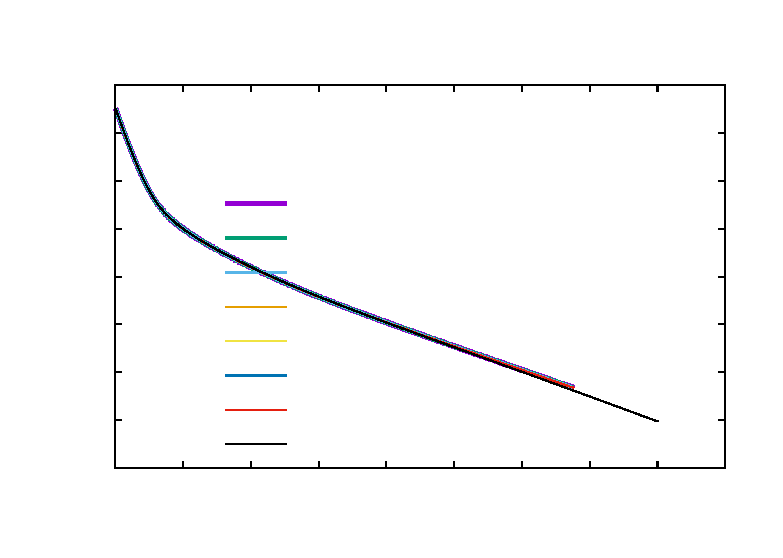
\includegraphics{viscos_rat=10_pos_diff}}%
    \gplfronttext
  \end{picture}%
\endgroup
